\documentclass[aspectratio=169,17pt]{beamer}

\usetheme{Madrid}
\usecolortheme{default}
\setbeamertemplate{navigation symbols}{}
\setbeamertemplate{footline}[frame number]

\usepackage[T1]{fontenc}
\usepackage[utf8]{inputenc}
\usepackage[brazil]{babel}
\usepackage{times}
\usepackage{booktabs}
\usepackage{tikz}
\usepackage{amsmath}
\usetikzlibrary{arrows.meta,positioning,shapes.geometric,fit}

\definecolor{uspblue}{RGB}{0,63,122}
\definecolor{usplight}{RGB}{232,241,250}
\setbeamercolor{structure}{fg=uspblue}
\setbeamercolor{title}{fg=white,bg=uspblue}
\setbeamercolor{frametitle}{fg=white,bg=uspblue}
\setbeamercolor{block title}{fg=white,bg=uspblue}
\setbeamercolor{block body}{bg=usplight}
\setbeamercolor{alerted text}{fg=uspblue}

\title[IA Melhora o Trading em Forex?]{O Sentimento Guiado por IA Pode Melhorar o Trading em Forex?}
\author[Wellington Souza]{Wellington Souza}
\institute[ICMC/USP]{MBA em Intelig\^encia Artificial e Big Data \\ ICMC, Universidade de S\~ao Paulo}
\date{S\~ao Carlos, 2026}

\begin{document}

\begin{frame}
  \titlepage
  \vspace{-0.6cm}
  \begin{center}
    \small Orientadora: Prof.\ Dr.\ Carolina Toledo Ferraz
  \end{center}
\end{frame}

\begin{frame}{Introdução e motivação}
  \begin{itemize}
    \item O mercado de câmbio reage a preço, liquidez, notícias e choques geopolíticos.
    \item Estratégias puramente baseadas em preço podem ignorar parte desse contexto.
    \item Este trabalho testa empiricamente se eventos de notícia acrescentam valor preditivo.
  \end{itemize}
\end{frame}

\begin{frame}{Objetivo e pergunta de pesquisa}
  \small
  \begin{itemize}
    \item \textbf{Objetivo}: desenvolver e avaliar uma estratégia híbrida de Forex com sinais de preço e eventos.
    \item \textbf{Pergunta}: a inclusão de eventos derivados de notícias melhora o desempenho frente a um \textit{baseline} somente de preço?
    \item Execução: intensidade de eventos GDELT; sentimento textual não foi avaliado.
    \item Resposta baseada em comparação pareada, configurações registradas e reprodução dos resultados.
  \end{itemize}
\end{frame}

\begin{frame}{Referencial teórico}
  \begin{itemize}
    \item Mercado Forex, custos de transação e avaliação fora da amostra.
    \item Aprendizado de máquina financeiro e risco de sobreajuste em backtests.
    \item NLP financeiro: sentimento como contexto teórico, eventos macroeconômicos e GDELT.
  \end{itemize}
\end{frame}

\begin{frame}{Metodologia: pipeline executado}
  \centering
  \begin{tikzpicture}[
    node distance=0.45cm and 0.35cm,
    pipebox/.style={draw, rounded corners, fill=blue!10, minimum width=2.1cm, minimum height=0.68cm, align=center, font=\scriptsize},
    arrow/.style={-{Stealth[length=2mm]}, thick}
  ]
  \node[pipebox] (data) {Dados};
  \node[pipebox, right=of data] (features) {Construção\\dos atributos};
  \node[pipebox, right=of features] (models) {Modelos\\utilizados};
  \node[pipebox, below=of models] (strategies) {Estratégias};
  \node[pipebox, left=of strategies] (evaluation) {Avaliação\\experimental};
  \node[pipebox, left=of evaluation] (stats) {Análise\\estatística};
  \draw[arrow] (data) -- (features);
  \draw[arrow] (features) -- (models);
  \draw[arrow] (models) -- (strategies);
  \draw[arrow] (strategies) -- (evaluation);
  \draw[arrow] (evaluation) -- (stats);
  \end{tikzpicture}
\end{frame}

\begin{frame}{Metodologia: avaliação}
  \begin{itemize}
    \item Três famílias de preço no \textit{baseline}; a estratégia híbrida acrescenta a família de eventos.
    \item Combinação final por regressão logística sobre probabilidades dos submodelos.
    \item Estratégias comparadas no mesmo período, com os mesmos custos e regras de execução.
    \item Controles adicionais distinguem rentabilidade aparente de capacidade preditiva.
  \end{itemize}
\end{frame}

\begin{frame}{Resultados e discussão}
  \begin{columns}[T]
    \column{0.48\textwidth}
    \centering
    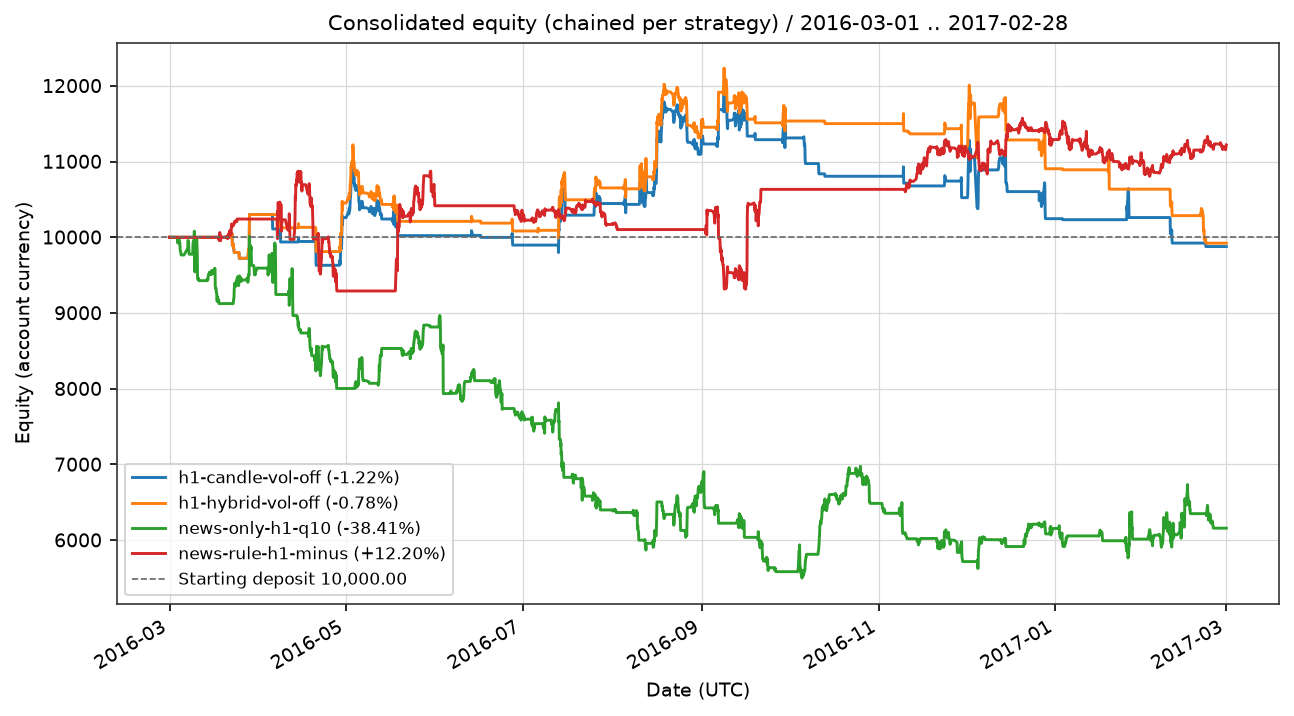
\includegraphics[width=0.95\textwidth]{img/equity-trading-year-h1.png}\\
    \tiny Março 2016 -- fev 2017, EUR/USD (janela registrada antes da simulação).
    \column{0.48\textwidth}
    \small
    \begin{itemize}
      \item \alert{Diferença pareada híbrido vs.\ baseline não significativa} ($p=0{,}149$).
      \item Resultado reproduzido com os mesmos números.
      \item Célula positiva = deriva (controle always-short, $p=0{,}92$).
    \end{itemize}
  \end{columns}
\end{frame}

\begin{frame}{Discussão dos resultados negativos}
  \begin{itemize}
    \item Uma rentabilidade positiva isolada não implicou capacidade preditiva.
    \item Limiares calibrados em um período curto não sobreviveram à mudança de regime.
    \item O sinal de notícias observado era de curto horizonte, enquanto a regra de saída mantinha posições por dias.
  \end{itemize}
\end{frame}

\begin{frame}{Resultados complementares}
  \begin{itemize}
    \item \textbf{Retreinamento adaptativo}: a política congelada perdeu $97.8\%$ no ano; as demais políticas ficaram para trabalhos futuros.
    \item \textbf{Catálogo de candlesticks}: o único padrão positivo foi indistinguível do acaso após controle de múltiplas comparações.
    \item \textbf{Notícias + candlestick}: o gate de concordância não tinha direção de notícia para confirmar o padrão.
  \end{itemize}
\end{frame}

\begin{frame}{Notícias e padrão positivo}
  \begin{columns}[T]
    \column{0.54\textwidth}
    \centering
    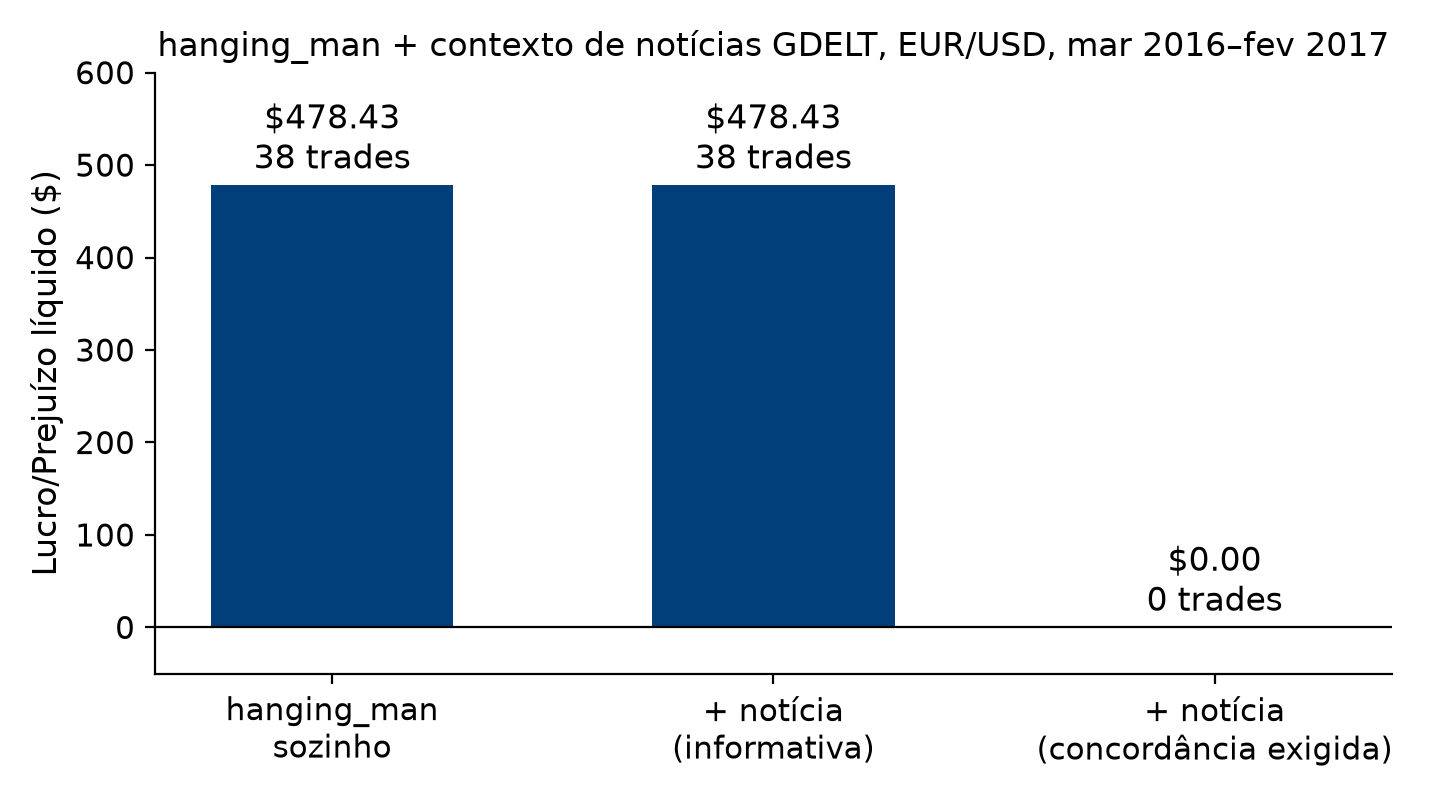
\includegraphics[width=\textwidth]{img/candlestick-news-combination-pt.png}
    \column{0.42\textwidth}
    \small
    \begin{itemize}
      \item Modo informativo: trades idênticos.
      \item Concordância obrigatória: zero trades.
      \item F4 se absteve em todas as barras elegíveis; não houve discordância ativa observada.
    \end{itemize}
  \end{columns}
\end{frame}

\begin{frame}{Conclusão}
  \begin{itemize}
    \item A pergunta de pesquisa, nesta configuração experimental, teve resposta negativa.
    \item O principal aprendizado científico é que retorno positivo aparente pode ser explicado por deriva e não por previsão.
    \item A contribuição empírica é um resultado negativo interpretável, reproduzível e auditado.
    \item A contribuição técnica é a infraestrutura de pipeline, replay e trilha de auditoria.
  \end{itemize}
\end{frame}

\begin{frame}{Limitações e trabalhos futuros}
  \begin{itemize}
    \item Limitações: uma janela principal, um par central e limiares escolhidos manualmente e nunca ajustados em dados fora da amostra.
    \item Componentes planejados, como sentimento textual, texto completo e fontes adicionais, não foram avaliados nesta versão.
    \item Trabalhos futuros: retreinamento adaptativo, cadeia de confluência, atributos intermercado e novos pares.
  \end{itemize}
\end{frame}

\begin{frame}
  \centering
  {\Large Obrigado. Perguntas?}
\end{frame}

\end{document}
